\documentclass[a4paper,12pt]{article}
\usepackage[T1]{fontenc}
\usepackage{polski}
\usepackage[utf8]{inputenc}
\usepackage[french,polutonikogreek,polish]{babel}
\usepackage{latexsym}
\usepackage{subfig}
\usepackage{graphicx}
\usepackage{sidecap}
\usepackage{wrapfig}
\frenchspacing

\begin{document}

\begin{titlepage}
\title{OBRAZY II - sprawozdanie}
\author{Michał Buszkiewicz, Rafał Mossakowski}
\date{20 XI 2014}
\maketitle
\end{titlepage}

\section{Wprowadzenie}
Celem naszego projektu było stworzenie oprogramowania ułatwiającego komunikacją człowieka z komputerem. Jego działanie opiera się na sterowaniu pozycją kursora w komputerze przy wykorzystaniu ruchów i gestów dłoni użytkownika. Do wykrycia obrazu posłużyła kamera dołączona do komputera oraz odpowiednie metody wchodzące w skład popularnej biblioteki do rozpoznawania obrazów - OpenCV. Wykonując odpowiednie gesty - np. poruszając otwartą lub zaciśniętą w pięść dłonią, użytkownik moze wydawać polecenia zmiany pozycji kursora lub kliknięcia. Tego typu rozwiązanie technologiczne mogłoby doprowadzić do powstania innowacyjnych interfejsów komputerowych, niewymagających urządzeń wskaźnikowych takich jak myszka czy touchpad.

\section{Wykorzystane techniki}
W związku z dużą ilością możliwych technik wykrywania dłoni oraz gestów na obrazie przesyłanym przez kamerę, byliśmy zmuszeni dokonać wyboru najwydajniejszej z nich na drodze eksperymentu. Po serii prób i błędów postawnowilismy wykorzystać metodę kaskadowych klasyfikatorów Chaara. Metoda ta opiera się na porównywaniu poszczególnych klatek odbieranego strumienia danych ze spacjalnym wzorcem, zawartym w pliku XML. Zastosowane zostały dwa różne wzorce: dla otwartej oraz dla zaciśniętej dłoni. Na obrazie wyświetlanym przez program, wykryte wzorce są oznaczane odpowiednio białym lub zielonym kwadratem. Ponadto, w specjalnym buforze przechowywana jest informacja, mówiąca czy w ostatnich dziesięciu klatkach wykryto otwartą czy zaciśniętą dłoń. Na podstawie jego zawartości podejmowane są odpowiednie akcje zdefiniowane w programie.



\section{Odrzucone techniki}
\subsection{Oddzielenie ręki przez progowanie}
Technika oddzielenia kształtu ręki przez progowanie jest ściśle powiązana z metodami służącymi do wykrycia krawędzi. Obraz wejściowy jest przetwarzany na skalę szarości - zgodnie z wymaganiami metod wykrywania krawędzi biblioteki openCV - po czym zostaje rozmyty z użyciem metody Gaussa w celu usunięcia zbędnych szumów, związanych z niską jakością obrazu. Następnie zostaje zastosowana metoda tzw. tresholdingu, czyli progowania. W efekcie uzyskiwany jest czarno-biały obraz, na którym wyraźnie widnieją kontury ręki. Po wykryciu wspomnianych konturów, obliczany jest związany z nimi centroiod. Zmiana położenia centroidu wskazuje na przesunięcie położenia ręki, co przekłada się na zmianę pozycji kursora. 
Przyczyną odrzucenia tego rzowiązania był fakt, iż jest ono mocno uzależnione od oświetlenia, w którym znajduje się kaera. Pinadto każdy obiekt widziany przez kamerę, niebędący jednocześnie ręką, ma negatywny wpływ na wykrywanie krawędzi - powoduje np. wykrycie "nieistniejących krawędzi".  
\begin{figure}
\centering
\subfloat[obraz wejściowy]{\label{odnosnik}
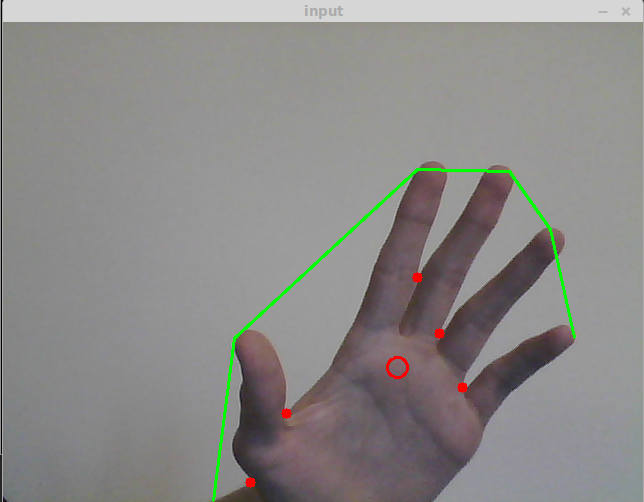
\includegraphics[width=0.45\textwidth]{sprawko_KCK1}}
\quad
\subfloat[obraz progowany]{\label{odnosnik}
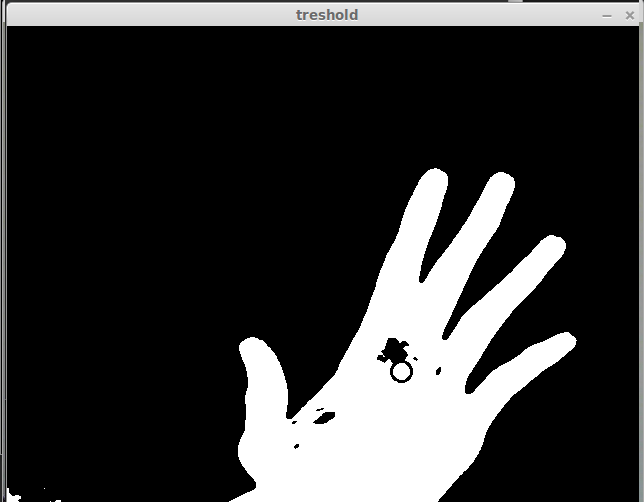
\includegraphics[width=0.45\textwidth]{sprawko_KCK2}}
\caption{Wykryeanie ręki przez progowanie obrazu}
\label{fig:animals}
\end{figure}

\subsection{Metoda próbkowania kolorów ręki}
Metoda próbkowania kolorów ręki jest metodą dwuetapową. W pierwszym etapie, użytkownik proszony jest o umiejscowienie ręki tak, aby była ona widoczna w specjalnym "kwadracie" zaznaczonym w oknie programu. Odpowiedni algorytm "próbkuje" wtedy kolor ręki. Po odpowiedniej kalibracji, program przechodzi do drugiego etapu, polegającego na zaznaczeniu konturów każdego elementu o kolorze podobnym do odczytanego koloru skóry użytkownika. W efekcie prowadzi to do zaznaczenia obszaru dłoni, co umożliwia dalsze sterowanie systemem komputerowym. Niestety rozwiązanie to jest obarczone pewnymi wadami. Największą z nich jest fakt, iż oprócz dłoni, zaznaczana jst także np. twarz użytkownika. Ponadto zmiana oświetlenia w trakcie pracy programu, może prowadzić do niezgodności pobranego początkowo wzorca koloru ludzkiej skóry z rzeczywistym odczytywanym kolorem.\\
Innym problemem w implementacji tego rozwiązania jest złożoność obliczeniowa - konieczność sprawdzenia każdego piksela ekranu w poszukiwaniu dopasowania kolorystycznego.\\
Przykład zastosowania tej metody obrazuje artykuł \footnote{Real –Time Hand Tracking and Gesture Recognition for Human-Computer Interaction, http://dmi.uib.es/~ugiv/papers/ELCVIAManresa.pdf}   


\section{Implementacja}

Działanie programu opiera się na analizowaniu każdej z klatek obrazu z kamery wideo pod kątem istnienia w niej dopasowań do wzorców (danych plikami XML klasyfikatorów kaskadowych): otwartej dłoni i zaciśniętej pięści.\\
W celu uproszczenia działania programu i odsiania błędnych odczytów, program filtruje wykryte dopasowania do wzorców, usuwając te, których wymiary są poniżej pewnego ustalonego progu (70x70 pikseli), a także bierze pod uwagę jedynie największą wykrytą na ekranie dłoń i pięść. Dodatkowo, jeżeli wykryte zostaną jednocześnie dopasowania do obu wzorców, program odrzuca dopasowanie otwartej dłoni, w celu ujednoznacznienia zachowania.\\
W celach poglądowych, wyświetlany jest obraz przedstawiający widok z kamery z nałożonymi prostokątami obrazującymi aktualnie wykryte dopasowania do wzorców.\\
Informacje o wykrytych przez program w ostatnich 20 klatkach dopasowania zapisywane są w buforze, na podstawie którego podejmowane są decyzje o akcjach i przejściach między stanami.\\
\\
Program w prezentowanej wersji operuje w kilku stanach. W zależności od stanu, w którym się znajduje, wykonuje różne akcje - taka budowa pozwala na łatwe rozszerzanie go o nowe reguły definiujące przejścia między stanami i zachowania w poszczególnych stanach. Aktualnie zaimplementowane stany:

\begin{itemize}
\item \texttt{waiting} - stan oczekiwania na sygnał przejścia w inny, aktywny stan. Powrót do niego następuje, gdy bufor ostatnich ramek zawiera jedynie ramki z brakiem dopasowań.
\item \texttt{fist} - stan pośredni, do którego przejście następuje poprzez utrzymanie przez 15 ramek zaciśniętej dłoni - z tego stanu można przejść w stan \texttt{cursor} poprzez utrzymanie następnie przez kolejne 5 ramek otwartej dłoni. Analogicznie można definiować inne przejścia do kolejnych stanów aktywnych.
\item \texttt{cursor} - stan sterowania kursorem myszy otwartą dłonią. W tym stanie program oblicza różnicę między aktualnym położeniem dopasowania dłoni w obrazie, a poprzednim wykrytym, wykorzystując ją do odpowiedniego przesunięcia względnego kursora myszy. Wartość przesunięcia kursora dana jest funkcją kwadratową, dzięki czemu szybsze ruchy dłonią powodują szybsze przesuwanie kursora. Dla najmniejszych wykrytych przesunięć dłoni tempo przesunięcia kursora jest dodatkowo spowalniane w celu zwiększenia precyzji kliknięcia.
\item \texttt{clicking} - utrzymanie przez dwie z trzech ostatnich ramek w stanie \texttt{cursor} zaciśniętej dłoni wprowadza program w stan \texttt{clicking}, który trwa tylko przez jedną klatkę. W tym stanie program wywołuje kliknięcie lewym przyciskiem myszy i od razu przechodzi w stan \texttt{cursor}.
\end{itemize}

\section{Możliwe usprawnienia}
Program można łatwo uzupełnić o dodatkowe przejścia między stanami i akcje im odpowiadające, poprzez dodanie kolejnych warunków w metodzie \texttt{do_action}.\\
Kilka możliwych do zaimplementowania funkcji to: sterowanie głośnością systemu, sterowanie odtwarzaczem multimedialnym, uruchamianie aplikacji określonym gestem, zmiana jasności ekranu.
\end{document}